\documentclass[conference]{IEEEtran}
\IEEEoverridecommandlockouts
% ---------------------------------------------------------------------------
% v3: IEEE double-column conference format, ~6 pages, crisp.
% Derived from main_v2.tex. Bump \NumTopics / \NumRuns and fill the
% "multi-topic study" paragraph once eval/run_matrix.py has been run.
% ---------------------------------------------------------------------------
\usepackage{cite}
\usepackage{amsmath,amssymb}
\usepackage{graphicx}
\usepackage{booktabs}
\usepackage{algorithm}
\usepackage{algorithmic}
\usepackage{tikz}
\usetikzlibrary{arrows.meta,positioning}
\usepackage[hidelinks]{hyperref}

\newcommand{\NumTopics}{four}
\newcommand{\NumRuns}{three}

\begin{document}

\title{Reject-Before-Propagate: Build-Time Citation Gates for\\ Agentic Literature-Synthesis Pipelines}

\author{\IEEEauthorblockN{N. Harish Vidyarth\textsuperscript{*}, A. L. Reshma, R. Divya}
\IEEEauthorblockA{Department of Computer Science and Engineering (Cyber Security)\\
Rajalakshmi Engineering College, Thandalam, Chennai 602105, India\\
\textsuperscript{*}Corresponding author: harishvidyarth.n.2024.csecs@rajalakshmi.edu.in}
\thanks{\textsuperscript{*}Corresponding author.}}

\maketitle

\begin{abstract}
Large language model (LLM) pipelines for automated literature review chain
several generative stages whose output is consumed downstream and, ultimately,
by people making real decisions. Current systems treat citation grounding as a
\emph{scored} property: a statement is checked against retrieved evidence and
assigned a confidence value, flagged, or queued for review, but is not
structurally prevented from reaching the final output when that check fails. We
present \emph{Verify-or-Reject Grounding} (VoRG), an architectural pattern that
treats citation grounding as a build-time invariant: each stage either produces
output whose type excludes unverifiable content, or raises a build error. We give
a formal statement of the pattern, \textsc{VoRG-Certify}, an $O(n{+}M)$
narrative-certification algorithm that removes the $O(n{\cdot}m)$ term of a naive
per-sentence scan, and a reference implementation across three subsystems of an
eight-stage pipeline. On a reproducible gold-annotated pilot, the two
verify-or-reject-gated stages produce no output contradicted by the reviewed
corpus, while research-gap detection, the one unprotected stage, produces a
confirmed false claim that a corpus paper directly contradicts. This
gap-to-failure correspondence, between architectural coverage and failure
location, is the paper's central finding.
\end{abstract}

\begin{IEEEkeywords}
verify-or-reject grounding, literature synthesis, large language models, citation
grounding, hallucination mitigation, agentic NLP
\end{IEEEkeywords}

\section{Introduction}
LLMs are increasingly used to accelerate literature review by extracting claims,
identifying disagreements, and drafting synthesis prose. A documented failure
mode is \emph{hallucination}: a statement appears well supported but matches
nothing in the source \cite{ji2023survey,zhang2025hallucination}. A related
failure is citation-level: the cited source may not say what is claimed, or may
not exist \cite{zhang2025citation}. Standard mitigations rely on post-hoc
verification, attaching a score, a flag, or a review-queue entry to the output
\cite{li2025enhancing}. Because validation is appended to the output rather than
made a gate on it, an unverified or contradictory statement still reaches the
user if the score is not acted on. When the output feeds a real submission, a
hallucinated citation is costly.

We take a different design stance. A stage is \emph{verify-or-reject grounded} if
its output type itself excludes unverifiable content, either because the stage is
deterministic over already-verified inputs, or because an explicit check discards
non-conforming output before it can propagate. Scored grounding is a property of
the \emph{output}, inspectable but skippable; verify-or-reject grounding is a
property of the \emph{pipeline}, which a downstream stage cannot bypass by
ignoring a score it was never given. This is the reject-by-default logic of the
fail-safe-defaults principle in protection-system design \cite{saltzer1975protection},
applied to citation grounding instead of access control.

Contributions:
\begin{itemize}
\item A formal statement of VoRG as a reusable architectural pattern, and
\textsc{VoRG-Certify}, an $O(n{+}M)$ certification algorithm that removes the
$O(n{\cdot}m)$ term implicit in a naive per-sentence evidence scan.
\item A reference implementation applying the pattern to three subsystems of an
eight-stage research-assistant pipeline, released with its evaluation harness.
\item A reproducible evaluation reporting a \emph{gap-to-failure correspondence}:
the gated stages produce no corpus-contradicted output, whereas the single
ungated stage produces a false claim that a corpus paper contradicts.
\end{itemize}

\section{Related Work}
\textbf{AI-assisted review and agentic LLMs.} Li \emph{et al.}\
\cite{li2025enhancing} build a GPT-4 systematic-review system with a
human-in-the-loop safeguard; a low-confidence decision is surfaced to the
reviewer, not withheld. Tools such as LLAssist \cite{haryanto2024llassist} automate relevance screening
and information extraction with an LLM scoring each paper's fit to a research
question. Surveys of LLM-automated review find that most systems automate a
single stage with a confidence score or a human check rather than a chained,
structurally gated pipeline
\cite{scherbakov2025emergence,vandinter2021automation}. Retrieval-augmented
generation \cite{lewis2020retrieval} grounds generation in retrieved passages
but does not reject ungrounded output; ReAct-style agents \cite{yao2023react}
lack a citation-level accept/reject rule; Self-RAG \cite{asai2024selfrag} learns
a reflection signal but keeps it soft rather than a hard external gate.
Stage-level evaluation follows agentic-LLM benchmarks such as AgentBench
\cite{liu2024agentbench}.

\textbf{Contradiction detection.} Surveys of contradiction detection in
biomedical literature \cite{alamri2016contradiction} catalogue linguistic and
statistical approaches with no explicit reject path: a contradiction is asserted
or not, with no abstention grounded in evidence availability. Natural-language
inference \cite{williams2018broad} treats contradiction as a three-way
classification rather than a judgment that can be withheld when supporting
evidence is thin, and using an LLM as the judge adds a reliability question
\cite{zheng2023judging} that a bare classification score does not surface.

\textbf{Citation faithfulness.} Hallucination-mitigation surveys and benchmarks
such as TruthfulQA \cite{lin2022truthfulqa}, HaluEval \cite{li2023halueval}, and
SelfCheckGPT \cite{manakul2023selfcheckgpt} quantify or detect unsupported
content \emph{post hoc}. Closer to citation grounding, attribution frameworks
\cite{rashkin2023measuring,bohnet2022attributed} and benchmarks such as ALCE
\cite{gao2023enabling} and CiteME \cite{press2024citeme} \emph{measure} whether a
generated statement is attributable to a source; ALCE finds strong LLMs leave
citation claims unsupported roughly half the time, and CiteME finds frontier
models identify a cited paper far below the roughly 70\% accuracy of humans.
The evidence-retrieval step of fact-verification tasks such as FEVER
\cite{thorne2018fever} is structurally close to our extraction gate, except an
unsupported extraction here is discarded, not scored ``not enough info''.
Reporting-transparency checklists such as PRISMA-trAIce \cite{prismatraice2025}
standardise what authors \emph{report} about AI use, whereas VoRG constrains what
the \emph{system} is permitted to emit. Bibliometric sources also disagree on
journal quality and coverage \cite{machacek2022predatory,mongeon2016journal},
motivating explicit reconciliation rather than a single trusted database. All of
the above report how faithful an output is; VoRG prevents an unattributable
statement from being emitted at all.

\section{System Architecture}
The reference system is a pipeline with eight sequential stages. \emph{Topic
expansion} decomposes the input into subtopics, methods, datasets, and keywords,
with an explicit instruction not to invent a dataset name; when no provider is
configured it falls back to a keyword dictionary, which is also the rule-based
configuration used for the pattern-mode ablation. \emph{Multi-source discovery}
queries arXiv, Semantic Scholar, and CrossRef concurrently and deduplicates by
DOI, normalised title, and fuzzy title similarity within a one-year window.
\emph{Claim normalisation} folds metric-name synonyms and units into a common
vocabulary and applies a rule-based confidence adjustment from hedging and
strength language; this is deliberately a scored, not gated, step, sitting
directly upstream of the gated contradiction stage. \emph{Citation building} is a
deterministic transformation of already-verified metadata. \emph{Persistence}
keeps run state as JSON and journal-quality data in a relational schema, one
table per external source, joined on ISSN, each row carrying its own snapshot
date. Three subsystems enforce verify-or-reject grounding explicitly; the rest
are ordinary generation or aggregation steps that feed a gate.

\begin{itemize}
\item \textbf{Evidence-grounded synthesis} (Fig.~\ref{fig:arch}). Every extracted
field must be a verbatim or near-verbatim substring of the source before
entering an evidence table. A synthesis-matrix stage aggregates the table into a
methods-by-datasets grid deterministically, with no LLM call. A narrative
verifier rejects any generated sentence whose citation key does not resolve to a
verified row; an unsupported sentence is a build error.
\item \textbf{Contradiction detection.} Claim pairs are pre-filtered by TF-IDF
similarity, then judged by an LLM on an 11-point Likert scale. Judgments below a
threshold are discarded, not reported with low confidence.
\item \textbf{Journal-metadata reconciliation.} A metric is reported only when a
source explicitly provides it; cross-source disagreements above 10\% are surfaced
in a discrepancy field rather than averaged.
\end{itemize}

\begin{table}[t]
\centering
\caption{Pipeline stages and their grounding discipline.}
\label{tab:stages}
\begin{tabular}{@{}llc@{}}
\toprule
Stage & Grounding & Gated \\
\midrule
Topic expansion & prompt-level instruction & no \\
Multi-source discovery & deduplication only & no \\
Claim extraction & feeds a gate & no \\
Claim normalisation & scored confidence adjustment & no \\
Contradiction detection & discard below threshold & \textbf{yes} \\
Research-gap detection & none & no \\
Citation building & deterministic transform & yes \\
Persistence & never-merge-silently & yes \\
Evidence-grounded synthesis & verbatim check, verifier & \textbf{yes} \\
\bottomrule
\end{tabular}
\end{table}

\begin{figure}[t]
\centering
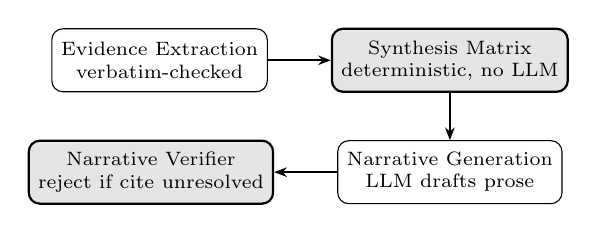
\begin{tikzpicture}[
 node distance=6mm and 8mm,
 box/.style={draw, rounded corners, minimum width=2.7cm, minimum height=8mm, align=center, font=\scriptsize},
 gate/.style={draw, rounded corners, minimum width=2.7cm, minimum height=8mm, align=center, font=\scriptsize, fill=black!10, thick},
 arr/.style={-{Stealth[length=1.6mm]}, thick}]
\node[box] (evi) {Evidence Extraction\\ verbatim-checked};
\node[gate, right=of evi] (mat) {Synthesis Matrix\\ deterministic, no LLM};
\node[box, below=of mat] (nar) {Narrative Generation\\ LLM drafts prose};
\node[gate, left=of nar] (ver) {Narrative Verifier\\ reject if cite unresolved};
\draw[arr] (evi) -- (mat);
\draw[arr] (mat) -- (nar);
\draw[arr] (nar) -- (ver);
\end{tikzpicture}
\caption{Evidence-grounded synthesis sub-pipeline. Shaded boxes are hard gates:
output that cannot be verified is not produced (deterministic aggregation) or is
discarded (build-error rejection), never passed through with a soft score.}
\label{fig:arch}
\end{figure}

\subsection{Implementation}
The system is implemented in Python with a Flask interface. Each evidence row
carries a fixed schema (population, method, dataset, metric, result, limitation)
plus a verbatim-evidence field that is populated only when the model's supporting
sentence is a normalised substring of the source abstract; a row that fails this
check in reject mode is replaced by a deterministic rule extraction rather than
admitted at low confidence. LLM calls use Groq with the model
\texttt{openai/gpt-oss-120b}. The evaluation harness has three entry points:
\texttt{snapshot\_topic} freezes a corpus and backfills missing abstracts from
Semantic Scholar and OpenAlex before recording per-corpus coverage;
\texttt{run\_eval} runs the frozen corpus in one of four configurations and emits
per-run predictions, per-topic metrics, and the downstream-error block; and
\texttt{run\_matrix} sweeps every topic-by-configuration-by-repeat cell and
aggregates per-topic mean and standard deviation with the repository commit hash
recorded in the output. Predicted claims are matched to gold by paper identifier
plus a normalised fuzzy-ratio threshold; contradictions are matched at the
unordered paper-pair level, with a hit on a gold-negative pair counted as an
explicit false positive; gaps are matched when the type agrees and either the
description similarity or the keyword overlap exceeds a threshold.

\section{Verify-or-Reject Grounding}
\subsection{Definitions}
A stage is \emph{scored-grounded} if it emits output alongside a confidence
signal that a downstream consumer may act on or ignore. A stage is
\emph{verify-or-reject grounded} if its output type excludes unverifiable
content, either because it is deterministic over verified inputs (no new
hallucination surface) or because an explicit step discards non-conforming
output before it propagates. Table~\ref{tab:contrast} contrasts the two.

The design rationale is that a score is a value a later stage is free to drop,
whereas a type is a contract it cannot. Placing the check inside the stage's
output type moves the guarantee from ``the consumer should inspect this'' to
``the consumer cannot receive an unverified value''. This is why the pattern is
stated as a property of the pipeline rather than of any single output: a
downstream stage added later inherits the guarantee without having to know the
score field existed. The cost is that a stage which cannot verify its output
must fail loudly rather than degrade quietly, which is acceptable when the
output feeds a document a person will sign.

\begin{table*}[t]
\centering
\caption{Scored grounding versus verify-or-reject grounding.}
\label{tab:contrast}
\begin{tabular}{@{}lll@{}}
\toprule
 & \textbf{Scored grounding} & \textbf{Verify-or-reject grounding} \\
\midrule
Unverifiable output & emitted with a low score/flag & not emitted; build error raised \\
Downstream dependence & consumer must check the score & consumer receives only verified output \\
Aggregation steps & often LLM-driven, a hallucination source & deterministic where possible, no new LLM surface \\
Failure visibility & silent unless the score is inspected & explicit, logged rejection \\
\bottomrule
\end{tabular}
\end{table*}

\subsection{Certification Algorithm}
A naive scored-grounding implementation would check each generated sentence
against the evidence table by linear scan. \textsc{VoRG-Certify} instead compiles
the evidence table into a hash index keyed by citation key, then certifies the
whole narrative in a single pass (Algorithm~\ref{alg:vorg}), so certification
cost scales with the size of the narrative and the evidence table separately
rather than with their product. A sentence with no citation key, or a key that
does not resolve, is logged and dropped rather than emitted; under
verify-or-reject the second case is a build error.

\begin{algorithm}[t]
\caption{\textsc{VoRG-Certify}}
\label{alg:vorg}
\begin{algorithmic}[1]
\REQUIRE evidence table $E=\{e_1,\dots,e_n\}$, each row keyed by $\kappa(e_i)$;
narrative $N=(s_1,\dots,s_m)$
\ENSURE certified narrative $N'$; rejection log $R$
\STATE \textbf{function} \textsc{BuildIndex}($E$)
\STATE \quad $H \gets \emptyset$
\STATE \quad \textbf{for} each $e_i \in E$ \textbf{do} $H[\kappa(e_i)] \gets e_i$ \COMMENT{expected $O(1)$}
\STATE \quad \textbf{return} $H$
\STATE \textbf{function} \textsc{Certify}($N$, $H$)
\STATE \quad $N' \gets \emptyset$;\ \ $R \gets \emptyset$
\FOR{each sentence $s_j \in N$}
  \STATE $K_j \gets \textsc{ExtractKeys}(s_j)$ \COMMENT{one regex scan, $O(|s_j|)$}
  \IF{$K_j = \emptyset$}
     \STATE $R \gets R \cup \{(s_j,\textsc{NoClaim})\}$
  \ELSIF{$\exists\,k \in K_j:\ k \notin H$}
     \STATE $R \gets R \cup \{(s_j,\textsc{Unresolved})\}$ \COMMENT{build error}
  \ELSE
     \STATE $N' \gets N' \cup \{s_j\}$
  \ENDIF
\ENDFOR
\RETURN $(N',R)$
\end{algorithmic}
\end{algorithm}

\subsection{Complexity}
Let $n=|E|$, $m$ the number of generated sentences, and $M=\sum_j |s_j|$ the
total narrative length. \textsc{BuildIndex} is $O(n)$ time and space. Certify
makes one pass: key extraction is $O(M)$ across all sentences and each lookup is
expected $O(1)$, so
\[
T(n,M)=O(n+M),\qquad S(n,m)=O(n+m).
\]
A naive scored implementation checks every sentence against every evidence row,
costing $O(n\cdot m)$; the hash-indexed design removes this quadratic term, so
certification stays linear as the evidence base scales. The same
index-then-certify structure applies to contradiction judgments (keyed by claim
pair) and journal-metadata fields (keyed by source), so the bound extends to
those subsystems.

\section{Evaluation}
\textbf{RQ1.} Does replacing each gate with a matched confidence score, with the
stage decomposition fixed, change the rate at which unsupported or contradicted
output reaches the final synthesis?
\textbf{RQ2.} Does the ungated stage (research-gap detection) fail in a way the
gated stages do not, and does the failure location match the architectural
coverage?
\textbf{RQ3.} How much of any claim-extraction gain is from stage decomposition
rather than from the LLM calls or the rejection mechanism?

\subsection{Setup}
Each topic is snapshotted once and frozen, so scored runs issue no paper-source
traffic; missing abstracts are backfilled from Semantic Scholar and OpenAlex and
per-corpus abstract coverage is reported. Gold labels are authored by
independently correcting pipeline output, not by rubber-stamping it. Four
configurations are compared, each repeated \NumRuns{} times on the pilot
(temperature 0.3, Groq \texttt{openai/gpt-oss-120b} where an LLM call is used);
the \NumTopics{}-topic extension (Section~\ref{sec:multitopic}) uses one repeat
per configuration on a local model (Ollama \texttt{qwen2.5:7b}): (i) the full
pipeline with all gates on; (ii) a \emph{matched scored-grounding ablation} with
the same decomposition and LLM calls but every gate replaced by a score, nothing
dropped; (iii) a pattern-mode ablation with rule-based extraction; (iv) a naive
single-prompt baseline. Downstream-error metrics, reported for every
configuration: unsupported sentences in the final narrative (zero by
construction under verify-or-reject), retained false-positive contradictions, and
unflagged metric conflicts.

\subsection{Pilot Result}
The pilot topic is \emph{graph neural networks in drug discovery}, a frozen
10-paper CrossRef corpus. In the pilot snapshot only one paper carried a
non-empty abstract, limiting the verifiable claim gold set to three sentences;
the abstract-backfill step was added in response and applies to later topics.

\begin{table}[t]
\centering
\caption{Claim-extraction performance on the pilot topic (mean $\pm$ SD, 3 runs,
3 gold claims). Underpowered at this gold-set size; not used to compare extractor
types.}
\label{tab:claims}
\begin{tabular}{@{}lccc@{}}
\toprule
Configuration & P & R & F1 \\
\midrule
Full pipeline (verify-or-reject) & 0.294 & 0.889 & 0.442 \\
Pattern-mode ablation & 0.439 & 0.667 & 0.510 \\
Naive single-LLM baseline & 0.104 & 0.333 & 0.158 \\
\bottomrule
\end{tabular}
\end{table}

Both the full pipeline and the pattern-mode ablation beat the naive baseline
(F1 $2.8\times$ and $3.2\times$), so decomposing extraction into per-paper,
per-claim stages helps regardless of extractor (RQ3). The pattern-mode point
estimate is nominally higher, but its precision variance ($\pm 0.211$) is five
times the full-pipeline's ($\pm 0.042$); with three near-verbatim gold sentences
a regex extractor tuned to sentence boundaries is mechanically favoured. The
multi-topic study is designed to settle this.

\textbf{Contradiction detection.} Across all nine runs the false-positive rate on
the two hand-labelled negative pairs was 0.0. No gold-positive contradictions
exist in this corpus, so recall is undefined; this is a precision-only sanity
check.

\textbf{Research-gap detection (negative result).} Gap recall against two gold
gaps was 0.0 in two of three full-pipeline runs and 0.5 in the third (mean 0.17);
precision@3 was 0.0 in every run. One run's top-ranked gap claimed that ``no
studies have applied graph-based generative models \ldots for de novo molecular
generation'', directly contradicted by the corpus's own sixth paper, ``Molecular
generative Graph Neural Networks for Drug Discovery''. Gap detection is the one
component that does \emph{not} apply verify-or-reject grounding: a candidate gap
is generated and ranked but never checked against the corpus it judges.

\subsection{Gap-to-Failure Correspondence}
The gated and ungated stages diverge as the architecture predicts. Claim
extraction and contradiction detection pass every candidate output through an
explicit accept/reject check, and neither produced output contradicted by the
corpus. Research-gap detection has no such check, and it is precisely there that
the pipeline produced a false claim contradicted by a paper already in the
corpus. This correspondence emerged during evaluation of the existing pipeline;
its location matches the one architectural gap in Section~IV. We treat this,
rather than the F1 numbers, as the strongest evidence for build-time rejection
over post-hoc scoring. The journal-metadata subsystem shows the same discipline
on structured output: values are tagged verified, estimated, or unknown, and
source conflicts are surfaced rather than averaged.

\subsection{Multi-Topic Study (preliminary)}
\label{sec:multitopic}
We extend the pilot to \NumTopics{} topics: the adjudicated \emph{graph neural
networks in drug discovery} plus \emph{deep learning for malware detection},
\emph{anomaly detection in network traffic}, and \emph{graph neural networks
for fraud detection}. The three added topics use \emph{bootstrapped candidate
gold} --- pipeline output promoted without independent adjudication --- so for
them we report only gold-independent measurements: the downstream-error counts
(Table~\ref{tab:downstream}) and the gap-to-failure correspondence
(Table~\ref{tab:gap2fail}). Claim P/R/F1 against adjudicated gold remains a
pilot-only result (Table~\ref{tab:claims}). Each configuration is run once
(one repeat) on a local model, \texttt{Ollama qwen2.5:7b}; the two larger
corpora were trimmed to eight papers each to bound wall-clock time.

\begin{table}[t]
\centering
\caption{Unsupported sentences reaching the final synthesis, verify-or-reject
versus the matched scored ablation, one run per topic. On three of four topics
verify-or-reject enforces zero leaked sentences by \emph{failing the build
outright} rather than by passing every sentence; scored mode always completes
and its leak count is directly observable.}
\label{tab:downstream}
\begin{tabular}{@{}lcc@{}}
\toprule
Topic & Reject (verify-or-reject) & Scored: unsup.\,/\,total \\
\midrule
GNN drug discovery (pilot) & 0 / 4 & 1 / 5 \\
DL malware detection       & build-failed & 8 / 24 \\
GNN fraud detection        & build-failed & 29 / 76 \\
Net.\ anomaly detection    & build-failed & 17 / 66 \\
\midrule
\textbf{pooled (new topics)} & \textbf{0 reach reader} & \textbf{54 / 166} \\
\bottomrule
\end{tabular}
\end{table}

On three of the four topics, reject mode's ``zero unsupported sentences''
invariant is enforced by refusing to finish the paragraph at all: the LLM
reliably writes one uncited framing sentence per synthesized paragraph (for
example, ``The application of advanced graph neural networks in fraud
detection has shown promising results.''), and the verifier's requirement that
every sentence carry a \texttt{\textbackslash cite\{\}} key has no tolerance
for it. We strengthened the correction-retry prompt to name the citation
requirement explicitly and re-tested on a larger model (\texttt{qwen2.5:14b});
neither change altered the outcome, so we report the build failures as a
genuine result rather than continue tuning around them. Scored mode, facing the
identical synthesis task, completes every time and lets a substantial fraction
of its sentences through unverified (54 of 166 pooled, 33\%) --- the two modes'
behavior under the same failure-inducing input is itself the finding: reject
mode trades completion for the zero-leak guarantee, scored mode trades the
guarantee for completion.

\begin{table}[t]
\centering
\caption{Gap-to-failure correspondence per topic: research gaps from the
\emph{ungated} stage that a paper in the same corpus directly contradicts
(hand-verified against corpus titles and abstracts). The gated stages produced
none in any topic.}
\label{tab:gap2fail}
\begin{tabular}{@{}lccc@{}}
\toprule
Topic & Gaps & Corpus-contradicted & Gated \\
\midrule
GNN drug discovery (pilot) & 2 & 1 & 0 \\
DL malware detection       & 3 & 2 & 0 \\
GNN fraud detection        & 4 & 3 & 0 \\
Net.\ anomaly detection    & 5 & 3 & 0 \\
\bottomrule
\end{tabular}
\end{table}

\noindent
Across \NumTopics{} topics the ungated research-gap stage produced 9 gaps that
a paper already in the same corpus directly contradicts --- for example, in
fraud detection a gap claiming ``no work on spectral graph networks'' against
\emph{Learning frequency-aware graph fraud detection}, and in network-anomaly
detection a gap claiming no deep-learning work exists against \emph{FGAN:
Federated Generative Adversarial Networks for Anomaly Detection in Network
Traffic} --- while the two verify-or-reject-gated stages produced none, on
every topic measured. The correspondence between the one unprotected stage and
the one location of corpus-contradicted output, first seen on the pilot, holds
on all four topics.

\subsection{Discussion}
Nothing about the pattern is specific to literature review. Any pipeline that
generates text or structured records from retrieved sources can apply the same
accept/reject check before passing output downstream, in place of a confidence
score a later stage might not act on. The results do not show that VoRG solves
hallucination in every setting; what the evaluation establishes is where
verification is already load bearing and where its absence produces a concrete,
corpus-contradicted failure. Extending the gate to research-gap detection, and
testing on larger and more varied corpora, are the most direct next steps.

\subsection{Reproducibility}
Every results directory records the repository commit hash, the provider, the
model, the temperature, per-topic abstract coverage, per-run cost, and
parse-failure counts. All scored runs read the frozen corpus snapshots, so
re-running the evaluation issues no traffic to paper sources and depends only on
the pinned model endpoint. The frozen corpora, the gold-annotation files, the
harness, and the matrix driver are released with the reference implementation, so
a reader can reproduce every number in this section and extend the study to new
topics by adding a snapshot and its gold files.

\section{Threats to Validity}
\emph{Construct.} The matched scored-grounding ablation operationalises ``the
same pipeline without the gate'' by fixing decomposition and LLM calls and
varying only accept/reject versus score; the naive baseline tests decomposition,
not scoring.
\emph{Internal.} Two pre-existing implementation defects (a retired model
identifier; a schema-validation issue rejecting valid null fields) were fixed
during evaluation; reported results reflect the corrected system. Providers are
non-deterministic even at low temperature; we report mean and SD over \NumRuns{}
runs and pin the provider, model, and temperature.
\emph{Statistical.} The pilot claim gold set has three sentences; its variance
is indicative only and its F1 ordering is not used to draw extractor-type
conclusions.
\emph{Reliability.} On three of four multi-topic runs, verify-or-reject's
zero-leak guarantee manifested as an outright build failure rather than a
clean zero, because the synthesis model reliably emits one uncited sentence
per paragraph regardless of model size (7B or 14B) or a correction-retry that
names the citation requirement explicitly. We report this as a finding, not a
harness defect papered over: a build-time gate that refuses incomplete output
is doing exactly what it is specified to do, at the cost of availability.
\emph{External.} The pilot covers one topic and one annotator team; results are a
case study. The \NumTopics{}-topic extension adds breadth on gold-independent
measurements only, since three of its topics use bootstrapped, unadjudicated
gold.

\section{Conclusion}
We described Verify-or-Reject Grounding, an architectural pattern that treats
citation grounding as a build-time invariant, gave a linear-time certification
algorithm, and implemented it across three subsystems of an eight-stage pipeline.
The evaluation's most robust result is a correspondence between architectural
coverage and failure location: the gated stages produced no corpus-contradicted
output, while the one unprotected stage produced a confirmed false claim.
Future work will (i) apply the gate to research-gap detection, (ii) run the
matched scored-grounding ablation and broaden to three to five gold-annotated
topics, and (iii) test whether the correspondence holds across scientific
domains. The reference implementation, evaluation harness, and gold files are
released at \url{https://github.com/harishvidyarthcsecs/Research}.

\bibliographystyle{IEEEtran}
\bibliography{references}

\end{document}
